\documentclass[12pt]{article}

\usepackage{fullpage}
\usepackage{graphicx, rotating, booktabs} 
\usepackage{times} 
\usepackage{natbib} 
\usepackage{indentfirst} 
\usepackage{setspace}
\usepackage{grffile} 
\usepackage{hyperref}
\usepackage{adjustbox}
\usepackage{amsmath}
\setcitestyle{aysep{}}


\singlespace
\title{\textbf{Alliance Participation, Treaty Depth, and Military Spending}}
\author{Joshua Alley\footnote{Graduate Student,
Department of Political Science, Texas A\&M University.}}
\date{{\normalsize \today}}

\bibliographystyle{apsr}

\begin{document}

\maketitle 

\doublespace 

\begin{abstract}
How does alliance participation affect military spending? 
Some argue that joining an alliance increases defense expenditures, while others contend that it produces spending cuts.
I argue that how alliance participation affects growth in military expenditures depends on the depth of military cooperation in the treaty. 
Security-seeking non-major powers often free-ride on their allies by reducing defense spending, but deeper alliances increase their military spending growth.   
Close military cooperation reduces the degree of free-riding by making the treaty more valuable and increasing the leverage of alliance partners. 
I test the argument by creating a measure of alliance treaty depth and employing it in a multilevel model. 
The research design generates new empirical evidence linking alliance participation and growth in state military spending from 1816 to 2007. 
I find that deep alliances increase growth in military spending from alliance participation in non-major powers relative to shallow treaties.  
This result helps scholars and policymakers better understand a central question about alliance politics that has been debated in scholarship for decades. 
\end{abstract}


 \newpage 


\section{Introduction}


Scholars of international relations have long acknowledged that there are two ways for states to increase their security. 
They can invest in indigenous military capability or form alliances \citep{Morgenthau1948, Altfield1984, Morrow1993}.
Because both policies provide security, broadly defined, alliance participation should change how states invest in military capability. 
But exactly how alliances influence military spending remains unclear. 


Existing scholarship produces contradictory predictions and evidence on the question of alliance participation and military spending. 
One view expects alliance participation will reduce military spending \citep{Morrow1993, Conybeare1994, DigiuseppePoast2016}. 
The other predicts alliance participants will spend more on defense \citep{Diehl1994, MorganPalmer2006}.
This paper addresses the divide by explaining when alliance participation leads to more or less defense spending. 
In doing so, it helps clarify a longstanding debate about alliance politics.


Debate between the two perspectives largely ignores heterogeneity among alliances,\footnote{See \citet{DigiuseppePoast2016} for an important exception.} which is essential to alliance politics scholarship \citep{Morrow1991, Leeds2003, LeedsAnac2005, Fordham2010, Mattes2012, Benson2012, Poast2013, Johnsonetal2015}.  
Given differences between treaties and states, alliance participation could plausibly increase or decrease defense expenditures. 
I emphasize the role of treaty depth to explain how alliance treaty participation impacts military spending. 


Deep alliances formalize extensive defense cooperation between partners.
Rather than make arms-length commitments, these treaties make unconditional promises of military support, promise aid, and obligate members to coordinate defense policy. 
For example, a 1963 alliance between Jordan and Iraq commits to military support as well as military aid, bases and institutions to govern military coordination. 


Adding treaty depth addresses free-riding, which is a salient threat to cooperation in alliances. 
Non-major powers are prone to free-ride, as they emphasize immediate security and have high opportunity costs of military spending. 
Because alliance participation provides extra security, it often reduces non-major power growth in military spending. 
Greater treaty depth attenuates that negative correlation between alliance participation and military spending among non-major powers by increasing allied leverage and treaty value. 
 

I employ a novel research design to test my argument.
First, I develop a latent measure of alliance treaty depth. 
I then incorporate that measure into a multilevel model which estimates how alliance treaty characteristics modify the impact of alliance participation on growth in military spending.
Multilevel modeling corresponds to the argument and generates useful comparisons between alliances. 
I fit the model on a sample of non-major power states from 1816 to 2007. 
I find that deeper alliances increase the impact of alliance participation on growth in non-major power military spending, relative to shallower treaties.


For non-major powers, deeper treaties provide more benefits at the cost of freedom to reduce military spending. 
This trade off illuminates a salient debate in US foreign policy about the costs and benefits of US alliances.
Advocates of deep engagement \citep{Brooksetal2013} and restraint \citep{Posen2014} in grand strategy have different views of alliances. 
Advocates of restraint argue that the United States should withdraw from many alliances, as allied states spend too little on defense, which increases US defense spending \citep{Preble2009}.
Proponents of continued deep engagement argue that the benefits of alliances exceed the costs, and the extent of allied free-riding is overstated \citep{BrandsFeaver2017}. 
Debates about how to respond to ``free-riding'' by US allies should consider the limited formal depth of most US treaties.
While my argument gives a partial accounting of alliance costs and benefits, it suggests adding or maintaining formal deep military cooperation could help check free-riding.   
US allies spend less on defense in part because the United States usually offers shallow formal alliance treaties. 
While limits on treaty depth limit entanglement abroad, they also constrain US leverage. 


The paper proceeds as follows. 
First, I summarize competing claims on alliance participation and military spending. 
Then I describe my argument in more detail. 
The third and fourth sections present the research design and results. 
The final section concludes with a discussion of the results and implications for scholarship and policy.  



\section{Do Alliances Increase or Decrease Military Spending?}


% quick intro and straight into it
Scholarship on alliance participation and military spending is divided between two views.
Each predicts a different average or unconditional effect of alliance participation by emphasizing one aspect of alliance politics.  
I start with the substitution and public goods logics connecting alliance participation with reduced defense spending. 


\subsection{Why Alliances Could Decrease Military Spending} 


These arguments begin with the premise that alliances and military spending both provide security.
The first such model treats security from an alliance as a public good. 
Olson and Zeckhauser argue that alliances are subject to a collective action problem \citep{OlsonZeckhauser1966}.
Because alliance security is neither rivalrous nor excludable, members contribute inadequate resources to collective defense. 
Alliance members can ``free-ride'' and smaller states exploit larger partners. 
Spending less allows alliance members to consume more non-defense goods, but the alliance provides suboptimal security.\footnote{\citet{SandlerForbes1980}, \citet{Oneal1990} and \citet{SandlerHartley2001} all modify the public goods logic while relying on Olson and Zeckhauser's core intuition.} 


Another argument that predicts reduced defense spending focuses on substitution between foreign policy instruments.
Substitution arguments recognize that states employ one policy in place of the other \citep{MostStarr1989}.
Alliances provide security without requiring additional military spending \citep{Morrow1993, Conybeare1994}. 
Given extra security, states rely on their allies and and reallocate military spending to other goods. 


Under substitution, allied military capability replaces other members' defense expenditures. 
DiGiuseppe and Poast refine the substitution logic by arguing that states will only reduce spending if the alliance is credible \citep{DigiuseppePoast2016}.
Because democracies make more credible commitments, they assert that defense pacts with democracies lower defense spending.
This conditional argument is a useful step towards bridging the theoretical debate. 


Both the substitution and public goods models expect that alliance participation reduces military spending due to opportunity costs of military expenditures. 
States have incentives to rely on their allies for security because spending more on the military leaves less for other goods \citep{Fordham1998, Fearon2018}.
On the other hand, a contradictory perspective asserts that alliance participation increases military expenditures. 


\subsection{Why Alliances Could Increase Military Spending}


Several arguments predict higher military spending by alliance members.
All share an intuition that states increase military spending to support their alliance commitments. 
In these models, investing in the military secures foreign policy gains from alliance participation. 


% ton of models- one sentance for each. add more detail later if needed. 
Diehl argues that alliances increase foreign policy obligations, necessitating extra military spending \citep{Diehl1994}.
Because alliances expand what a state can achieve in international relations, states increase military spending to pursue other foreign policy goals \cite{MorganPalmer2006}.
For example, buffer states increase defense effort to make themselves a more attractive alliance partner \citep{Horowitzetal2017}.
Others assert that alliances generate cooperation, leading to higher defense spending \citep{Palmer1990, QuirozFlores2011}. 
These predictions of a positive correlation between alliance participation and military spending contradict the prediction of lower military spending by allied states.\footnote{
\citet{SeneseVasquez2008} argue that military spending and alliances are part of a conflict spiral of simultaneous growth in military expenditures and alliance participation. 
This argument suggests that any correlation between alliances and military spending is driven by conflict behavior, not treaty participation.
}


\subsection{Mixed Evidence} 


Debate between the contradictory views of alliances could be settled by a consistent set of average effects, but mixed results reinforce the theoretical division.
Some studies find a positive association between alliance participation and military spending. 
Others find a negative relationship.\footnote{
Because tests of the public goods model use military spending as a share of GDP as the their outcome of interest, I ignore most of those results.} 


% Specific and general studies
General studies of military spending and alliances compare many states through dummy indicators of alliance participation, which combine alliances into a state-level measure. 
This design compares states with an alliance to those without.
\autoref{tab:results-sum} summarizes previous results from general models of alliance participation and military spending. 
There is one negative, three positive and two null estimates of the correlation between alliance participation and spending. 


\begin{table}[hbt!]
\begin{center}
\begin{tabular}{lccc}
     & Decrease & Increase & Null \\
\hline
\citet{MostSiverson1987} &  &  & X \\
\citet{Conybeare1994} & X & &  \\
\citet{Diehl1994} &  & X &  \\
\citet{Goldsmith2003} &  &  & X \\
\citet{MorganPalmer2006} &  & X & \\ 
\citet{QuirozFlores2011} &  & X &  \\ 
\hline
\end{tabular}
\caption{General Findings of Association Between Alliance Participation and Military Spending.}
\label{tab:results-sum}
\end{center} 
\end{table}


% Virtues and shortcomings- Specific studies of substitution theory of FP 
Unlike general studies, specific research designs examine individual treaties and estimate responses to military spending of key allies. 
Most evidence of reduced military spending by alliance members comes from alliance-specific research designs \citep{BarnettLevy1991, Morrow1993, Sorokin1994, PluemperNeumayer2015, GeorgeSandler2017}.
Other specific studies find increased spending by alliance members, however \citep{ConybeareSandler1990, Chenetal1996}. 


\subsection{The Theoretical Challenge}


The mixed empirical results reflect a theoretical problem. 
Both perspectives make unconditional claims about the average effect of alliance participation on military spending.  
With one exception \citep{DigiuseppePoast2016}, scholarship on alliance participation and military spending ignores differences between alliances.
Treaty obligations vary widely across alliances \citep{Leedsetal2002}, which leads to heterogeneous effects. 
Conflict \citep{Leeds2003, Benson2012} and trade \citep{Long2003, LongLeeds2006} are two domains where alliance design shapes the impact of treaty participation. 


Differences in alliance treaty design should lead us to question binary measures of alliance participation in general studies and limit the generalizability of inferences from specific studies. 
Alliance participation could increase or decrease military spending, depending on treaty obligations. 
While \citet{DigiuseppePoast2016} focus on the conditionality of alliance credibility based on democratic membership, I look at the depth of cooperation in the treaty. 


My argument focuses on treaty depth as an important source of heterogeneity in how alliance participation impacts military spending. 
Formal treaty depth alters the consequences of alliance participation for non-major powers by limiting their ability to reduce defense spending. 
The next section summarizes the argument in more detail. 



\section{Argument}

% outline the whole argument
Deep military cooperation in an alliance reduces non-major powers' tendency to free-ride by increasing allied leverage and making the treaty more valuable. 
Non-major powers have less freedom to reduce defense spending under greater influence from their partners. 
As for treaty value, inadequate defense spending could antagonize partners into reducing or eliminating a valuable commitment. 
Therefore, non-major power growth in military spending from alliance participation is higher in deep treaties, relative to shallow ones. 


% Summarize the flow of the argument
I start the argument by describing problems of opportunism and enforcement in alliances. 
Then I describe the role of deep formal military cooperation. 
Last, I show how alliance depth attenuates the tendency of alliance participation to reduce growth in non-major power military spending. 


\subsection{Free-Riding in Alliances}

% opportunistic behavior in alliances and international cooperation 
Alliances are a form of international cooperation. 
By promising to aid one another in war, states make a credible commitment of intervention \citep{Fearon1997, Morrow2000}. 
Allied support helps members achieve crucial foreign policy goals like deterrence or success in war \citep{Walt1990, Snyder1997}. 


% Can think about this as an enforcement problem
Like all cooperation, alliances can suffer from opportunism, or ``behavior with guile'' \citep{Williamson1985}. 
Even as states commit to an alliance, they can also benefit from defecting and taking advantage of allied cooperation. 
Sometimes the perceived benefits of defection outweigh the long-run benefits of cooperation, so alliance members face an enforcement problem \citep{Fearon1998a, Koremenosetal2001}.


% Problem of allied states not spending enough on the military: 
Free-riding through low defense spending is one form of opportunism in alliances.\footnote{Though the public goods model of alliances has serious theoretical and empirical flaws, it is common practice to describe low defense spending in an alliance as free-riding.}
Though states contribute to the collective military capability of an alliance through their military spending, they can also reduce defense spending and rely on their partners \citep{OlsonZeckhauser1966, Morrow1993, Conybeare1994, SandlerHartley2001}.
Reduced defense spending can be a form of shirking that leaves allied states bear a greater military burden. 


Enforcing cooperation around free-riding is difficult.\footnote{See \citet{Poast2012, Poast2013} and \citet{LongLeeds2006} on how issue linkages address abandonment, which is another salient form of opportunism in alliances.}
Normative appeals to common interests rarely work. 
Though verbal communication or ``cheap talk'' can have value in international politics \citep{Trager2010}, it is unlikely to overcome incentives to free-ride. 
Even when they spend less on the military, alliance members retain foreign policy benefits and can reallocate resources to other priorities. 
The ability to reduce defense spending and spend more on other social goods sometimes motivates states to form alliances \citep{Kimball2010, AllenDigiuseppe2013}. 


% Transition- depth of military cooperation is a solution
Deep alliances provide two mechanisms that address incentives to free-ride. 
Stipulating deep cooperation increases both allied influence and the value of the alliance. 
As a result, members have less freedom and motivation to reduce defense spending. 



\subsection{Depth of Military Cooperation} 


% Define depth again 
Alliance depth is the extent of defense cooperation formalized in the treaty. 
There are two sources of depth. 
The first primary obligations: what support the alliance promises and when it applies. 
Formal peacetime defense cooperation is the second source of depth. 
In general, deep alliances stipulate close cooperation between members.
By contrast, shallow alliances promise more arms-length cooperation. 


% Conditions/circumstances the alliance covers and what is promised 
The primary obligations of the alliance add depth by stipulating how and when the treaty applies. 
Less than half of alliances promise military support. 
Commitments of non-aggression, neutrality or consultation are minimal, arms-length obligations. 
Defensive or offensive commitments of military intervention, by contrast, require closer cooperation to manage the alliance \citep{Snyder1997}. 
Promises of military support are a key source of depth. 


Besides military support, depth comes from conditions on primary obligations. 
Conditional alliances limit military intervention to specific circumstances. 
For example, an alliance may only promise defensive intervention if the fighting was unprovoked or involves a specific state.  
Alliance members use conditions to address moral hazard problems in alliances \citep{Benson2012, Bensonetal2014} and manage their own obligations \citep{Chibaetal2015}. 
Conditional obligations reduce the depth of the alliance by by limiting when members must cooperate. 
Unconditional alliances apply to many circumstances, increasing the extent of defense cooperation between members.


% ties between the partners 
Beyond the core obligations and conditions, states add depth to alliances by incorporating promises of peacetime defense cooperation. 
This cooperation takes many forms. 
Allies can form an integrated military command, provide military aid, commit to a common defense policy, provide basing rights, set up a formal organization to manage the alliance or undertake companion military agreements. 
All of these obligations move alliance members away from an arms-length partnership towards close cooperation via policy coordination and regular interaction. 


Increasing military coordination adds ties between alliance members beyond a promise of military support, which adds substantial depth. 
One example of a deep alliance is a 1948 defense pact between the United Kingdom and Jordan, which includes unconditional military support, basing rights, military aid, official military contact, and an Anglo-Transjordan Joint Defense Board.  
This is a deeper alliance than a 1912 alliance between Greece and Bulgaria which only commits to mutual defense and consultation if either state is attacked by Turkey. 


Alliance depth is a mechanism to reduce free-riding. 
Depth restricts the ability of members to free-ride in two ways. 
Adding depth to an alliance gives partners more leverage and increases the value of alliance participation. 


% implication 1: allies lose some residual control- partners have more influence
Partners have more influence in a deep alliance because defense cooperation provides leverage. 
Common defense policies, military aid, international organizations, aid and bases provide multiple avenues to check free-riding. 
Such treaty promises also generate peacetime obligations. 
Deep alliances require coordination and military effort even when members are not at war. 
This shapes the division of effort among alliance members and leaves less scope for free-riding. 


% Lake 1996- residual control 
Deep cooperation also aligns defense policy across issues beyond formal treaty content. 
As depth increases, the nature of the relationship the alliance codifies changes. 
Arms-length relationships are more anarchic, while close cooperation is often more hierarchical. 
In hierarchical relationships, partners give up control on issues beyond those the treaty formally addresses. 
\citet{Lake1996} calls this a loss of residual control, where one partner gives up control over issues outside the formal agreement. 
Deep alliances often reflect past territorial control, attempts to form federations, or wartime coalitions, all of which are more hierarchical than arms-length agreements among equals. 


As a result, deep treaties give alliance partners more influence over issues like military spending.
Inasmuch as allies understand this arrangement, direct coercion over free-riding will be rare in deep alliances.  
Additional leverage is not the only check on free-riding, however. 


% implication 2: alliance is more valuable
Members of deep alliances also lose some motivation to reduce defense spending because deep cooperation is valuable. 
Besides military support, members benefit from policy coordination and transfers. 
Depth increases the foreign policy benefits of alliance participation by helping members coordinate policy stances and defense effort.
This facilitates members' pursuit of common interests in international relations \citep{Snyder1997}. 


Because deep alliances are more valuable, members are less likely to free-ride. 
Insufficient defense spending could antagonize allies and lead them to abandon the alliance. 
Free-riding in a deep alliance endangers more than a promise of military support, it imperils close defense cooperation. 
This value logic is similar to issue linkages, where failure to cooperate on one dimension threatens valuable cooperation on another issue. 
In deep alliances, failure to spend enough on defense endangers other military cooperation with allies, not just their promise of military support. 


% so why not all deep, all the time?- Concerns about foreign entanglement/lost freedom of action
If deep alliances are a valuable source of influence over allied behavior, why are many alliances shallow? 
Depth in an alliance comes at the cost of foreign entanglement. 
In general, alliance members sacrifice some of their freedom of action in foreign policy in return for the benefits of alliance participation \citep{Altfield1984, Snyder1997}.
Deeper military cooperation sharpens this trade off between benefits and foreign policy freedom. 
Shallow alliances provide fewer direct benefits, but they also have less foreign entanglement.\footnote{Also deep alliances do not solve every problem, as more institutionalized alliances may not be more reliable \citep{LeedsAnac2005}.}
Domestic politics \citep{Davis2004}, democracy \citep{Chibaetal2015} and a state's international reputation \citep{Mattes2012} may all lead to more arms-length cooperation and shallow treaties. 


% Credibility objection
Another objection to the above argument is that deep alliances should be more credible, which allows alliance members to reduce defense spending \citep{DigiuseppePoast2016}. 
Although deep alliances provide more foreign policy benefits, added benefits are paid for with less freedom of action. 
In bargaining among alliance members, depth indicates members are willing to undertake obligations to receive foreign policy benefits \citep{Weber1997}.  
Other sources of credibility, such as allied democracy, do not come with extra obligations. 
By increasing allied leverage and treaty value, treaty depth connects security benefits with other costly cooperation. 


Shallower alliances still provide security by addressing crucial issues. 
Moreover, credibility is multifaceted. 
Alliance members employ multiple sources of credibility, based on their tolerance for the costs, benefits and risks of depth. 
Therefore, shallow alliances are not necessarily incredible, which allows members to reduce defense spending.  


% Transition- consequences for free-riding
In summary, deep alliances restrict free-riding among alliance members. 
This is especially relevant for non-major powers.
These states are more likely to free-ride. 


\subsection{Deep Cooperation and Non-Major Powers} 


% Use tradeoff models to explain that non-major powers are especially likely to free ride 
Non-major powers have limited military capabilities and less status in international relations. 
As a result, they usually focus on ensuring their immediate security.  
The emphasis on security creates opportunities for exchanges where non-major powers trade foreign policy autonomy for allied protection \citep{Altfield1984, Morrow1991}. 
By giving non-major powers more security, alliances allow them to reduce defense spending. 


% Gain high opportunity costs of military spending  
Besides their security goals, non-major powers face higher opportunity costs of military spending. 
The marginal cost per taxpayer of increases in defense spending is decreasing in the number of taxpayers \citep{DudleyMontmarquette1981}, and non-major powers have fewer taxpayers. 
Small states also have limited economies of scale in military spending \citep{Moravcsik1991, Kapstein1991, Anderton1995, Devore2013}.
These economic factors and non-major powers' foreign policy goals encourage free-riding.  


% Depth restricts ability of non-major powers to free-ride
Alliance participation often reduces non-major power defense spending. 
Greater alliance treaty depth attenuates this negative correlation, however. 
Allied leverage and treaty value can overcome non-major power incentives to free-ride. 


To illustrate the logic, consider two related alliances from the inter-war period. 
In 1925, France and Poland formed a defense pact promising military support in the event of an unprovoked German attack (ATOPID 2135). 
The treaty contained no other obligations and provided enough security for Poland to reduce growth in their defense budget.
On the other hand, a 1920 treaty between France and Belgium (ATOPID 2055) added commitments of military aid and a coordinated occupation of the Rhineland to defensive obligations. 
Belgian obligations exceeded defense in war, so the Franco-Belgian treaty increased growth in Belgian military spending. 
 
 
These brief examples and the argument suggest that treaty depth modifies the impact of alliance participation on non-major power military spending. 
Alliance participation is expressed not through allied capability, not just the presence of a treaty. 
Non-major powers free-ride on allied capability, so my measure of alliance participation uses allied capability to capture the effect of participation. 
Greater depth increases the usual negative impact of alliance participation on non-major power military spending. 
Deeper alliances will lead to higher growth in non-major power military spending than shallow treaties. 
 

\begin{quote}
\textsc{Hypothesis 1: As alliance treaty depth increases, growth in non-major power military spending from alliance participation will increase.}
\end{quote}



\subsection{Interpreting Predictions about Spending Growth}


When treaty depth increases growth in non-major power spending, the level of military spending may only change in a counterfactual sense. 
Higher expenditure growth need not produce larger defense budgets. 
Only positive growth in spending increases the level of military expenditures. 
When increasing growth in military spending remains negative, spending levels will fall. 


For example, a non-major power whose military budget goes from \$10 million to \$9 million due to an alliance experiences -10\% growth in spending. 
If the same alliance had greater depth and spending decreased from \$10 million to \$9.5 million, growth falls to -5\%, but the level still falls. 
Therefore, my arguments about growth apply to the level of military spending through counterfactual reasoning \cite{Fearon1991}. 
Increasing growth implies a state would have spent less on the military, all else equal.


\begin{figure}[htbp]
	\centering
		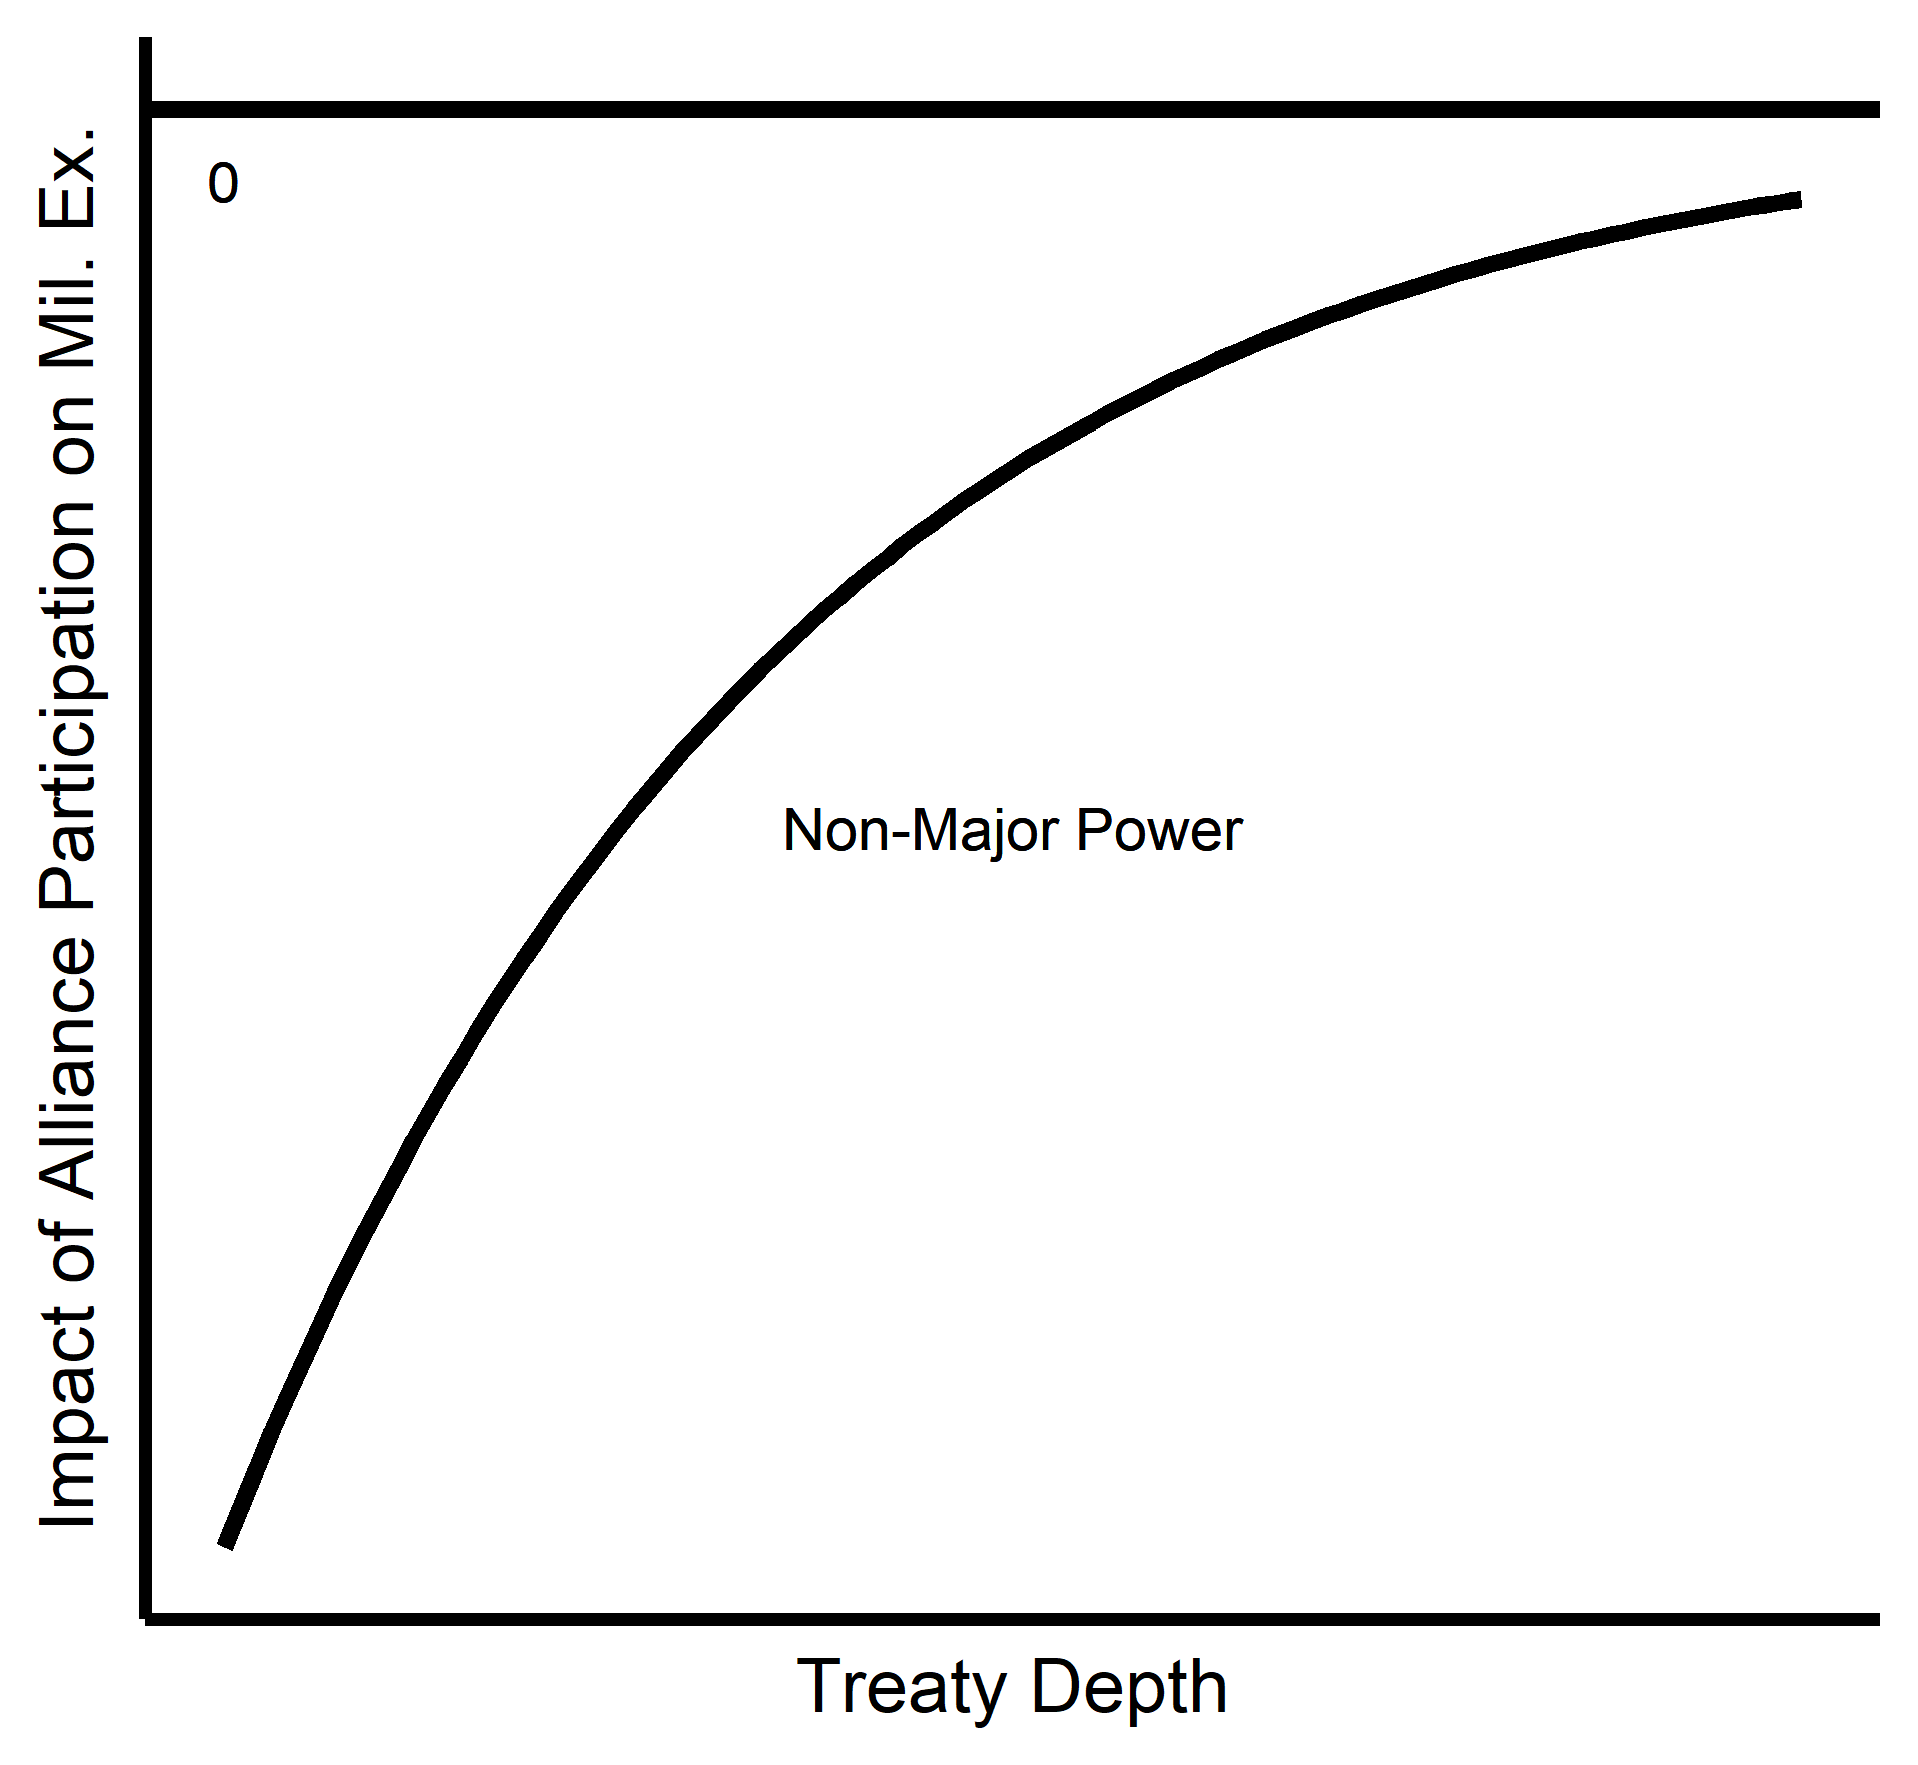
\includegraphics[width=0.95\textwidth]{../figures/illus-arg.png}
	\caption{Abstract illustration of the link between treaty depth and the impact of alliance participation on military spending.
	The curve represents a possible impact of alliance participation on growth in non-major power military spending across the range of treaty depth.}
	\label{fig:illus-arg}
\end{figure}


\autoref{fig:illus-arg} illustrates a possible implication of treaty depth about military spending by plotting a hypothetical link between treaty depth and the impact of alliance participation on military spending. 
The shape and level of the curve are not essential to the argument--- growth in non-major power military spending could be positive at high levels of treaty depth. 
\autoref{fig:illus-arg} only shows the need to be careful moving from changes in spending growth to changes in levels. 


For non-major powers, higher growth in spending in a broad treaty depth could remain negative. 
Deep treaties attenuate the negative correlation between alliance participation and military spending in non-major powers. 
But so long as growth from alliance participation remains negative, the level of military spending will fall. 


% Transition para
Because my argument focuses on differences between deep and shallow treaties, the research design must measure alliance treaty depth and compare alliances.  
I use a measurement model to infer treaty depth from formal content, then connect alliances to military spending with a multilevel model. 
The next section describes the research design in more detail. 



\section{Research Design} 


% two contributions: Develop latent str. measure and then put it into an ML model
The research design makes two contributions. 
First, I develop a latent measure of alliance treaty depth. 
Second, I employ that measure in a multilevel model, connecting alliance-level variation with state-level outcomes. 
I estimate the multilevel model in a sample of non-major powers from 1816 to 2007. 
The next section describes the measure of alliance treaty depth. 


\subsection{Measuring Alliance Treaty Depth} 


% Intuituion behind latent measures: observed char reflects underlying concept
Observed alliance commitments reflect the underlying depth of the treaty. 
Deep treaties promise more military cooperation. 
Therefore, I use observed alliance characteristics to infer treaty depth.


Using observed treaty conditions as indicators of underlying depth could produce two measures. 
One possible measure is an additive index of treaty depth, where treaties with multiple commitments have higher index values. 
This assumes each indicator is equally important, which is unlikely. 
Instead, I employ latent variable modeling, which is a more flexible way to use observable characteristics to infer an underlying trait.  
The measurement model estimates the correlations between alliance treaty content and the underlying formal depth to predict the depth of each treaty. 


% Justify use
Measurement models have a rich history in political science \citep{Clintonetal2004, TreierJackman2008, Fariss2014}.
Benson and Clinton use a mixed factor analysis model to measure alliance scope, depth and capability \citep{BensonClinton2016, Quinn2004}.  
I emulate Benson and Clinton's approach, but employ different indicators of depth and another estimator. 


% How the model works
I use a Bayesian Gaussian Copula Factor Model \citep{Murrayetal2013} to measure alliance treaty depth. 
Murray et al's model improves inferences from mixed factor analysis for continuous, ordinal, and binary observed data by relaxing distributional assumptions. 
Given discrete observed variables and non-Gaussian latent variables, the dependence among the latent variables and their marginal distributions are both influenced by the latent variables.
This model breaks the dependence between the latent factors and marginal distributions by using copulas to encode the dependence among the latent variables.\footnote{Copulas are a distribution function on $[0, 1]^p$ where each univariate marginal distribution is uniform on [0, 1].}


Beyond the semiparametric aspect, this measurement model is a standard mixed factor analysis.
Factor analysis estimates the association between observed variables and some latent factor.
Each observed variable has a factor loading--- the association between the observed variable and the latent variable.  
Like standardized regression coefficients, factor loadings range from -1 to 1, so observed variables are positively or negatively correlated with the latent factor.  
For each observation, a linear combination of observed alliance characteristics predicts latent treaty depth, like a regression with an unobserved outcome.  


I estimated the model using observed data from all 745 alliances in the alliance-level ATOP data \citep{Leedsetal2002}. 
Indicators of treaty depth are divided between the primary obligations and additional cooperation.
Primary obligations include promises of defensive support, offensive support, neutrality, consultation, non-aggression and whether military support is unconditional. 
I created the indicator of unconditional military support using ATOP data on whether offensive or defensive promises in the alliance are conditional on specific circumstances. 
Promises of defensive or offensive support, especially unconditional obligations, require deeper defense cooperation than arms-length promises of consultation, neutrality or non-aggression. 
Indicators of defense cooperation include military aid, bases, international organization formation, integrated military command, defense policy coordination and commitments to form companion military agreements. 
The argument suggests there is a single factor underlying variation in all 11 indicators, so I fit the model with one latent factor. 


I used Parameter expanded Gibbs sampling, the default generalized double Pareto (GDP) prior, 20,000 burn-in iterations of the MCMC chain, and 30,000 samples thinned every 30 observations to ensure convergence. 
The estimates include posterior distributions for the factor loadings and the latent factor. 
Because treaty depth is the quantity of interest, I focus on the posteriors of the latent factor. 


% Show the measure for all alliances- note I'll only focus on treaties w/ military support.
Each alliance has a unique posterior distribution of its latent depth. 
I use the mean of that posterior to measure treaty depth. 
\autoref{fig:ld-summary} describes the latent measure for ATOP alliances with defensive or offensive commitments from 1815 to 2016.
I examine the 289 alliances with military support because prior studies of alliance participation and military spending emphasize these treaties.\footnote{
I estimated the measurement model on all alliances, including those without military support to capture the contributions of primary obligations to treaty depth.}
The posterior mean captures the expected depth of an alliance treaty, conditional on its formal promises. 


There is substantial variation in the depth of alliance treaties. 
The top panel of \autoref{fig:ld-summary} is a histogram of mean treaty depth for alliances promising military support.  
Most treaties are concentrated between .5 and 1.5 on the latent scale, but approximately 40 treaties fall outside this range. 
The bottom panel of \autoref{fig:ld-summary} plots the posterior means and uncertainty in those estimates against the start year of the treaty. 
Even after accounting for uncertainty, it is possible to distinguish between some alliances. 


\begin{figure}
	\centering
		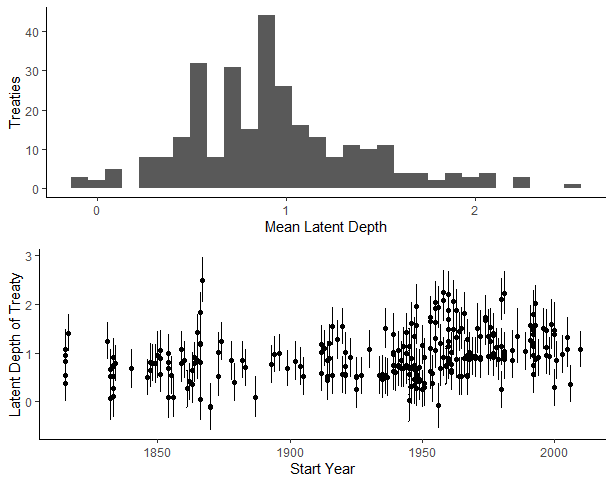
\includegraphics[width=0.95\textwidth]{../figures/ld-summary.png}
	\caption{Summary of latent measure of alliance treaty depth for 289 alliances promising military support from 1816 to 2016. The top panel is a histogram of the expected of alliance treaty depth. The bottom panel plots mean treaty depth (points) and the standard deviation (error bars) against the start year of the treaty.}
	\label{fig:ld-summary}
\end{figure}


% Cases- especially deep and shallow treaties
Although the values of the latent measure are not intrinsically meaningful, differences between treaties on the latent scale are informative. 
The mean of treaty depth is 0.92, and the median is 0.89. 
The median treaty is a 1967 agreement between Czechoslovakia and East Germany (ATOP ID 3550). 
Two of the most shallow treaties are twin 1870 neutrality and offense pacts, one between between France and Britain (ATOPID 1300), and the other between Prussian and Britain (ATOPID 1295).\footnote{
Sampling variation produces small differences in the scores. These alliances do not enter the later test, as they only involve major powers.} 
Britain used these alliances to protect Belgian neutrality during the Franco-Prussian war.  
Both treaties have only offensive and neutrality promises, conditional on France and Prussia respecting Belgian neutrality. 


NATO (ATOPID 3180) has a mean latent depth of 0.69, placing it just above the first quartile of military alliances. 
NATO's two costly provisions are the conditional defense obligations in Article 5 and establishing the Atlantic Council. 
According to the ATOP coding sheet for NATO, ``There are numerous bilateral agreements among NATO members re: military aid, bases, etc. but they do not qualify as separate alliances, nor are they part of the overall NATO structure.''
The NATO treaty is below average in formal depth in part because additional commitments fall outside the formal treaty.    


The three deepest treaties are an 1867 alliance between Prussia and Hesse (ATOPID 1290), a 1958 alliance between the UAE and Yemen (ATOPID 3345), and a 1981 pact between Gambia and Senegal. 
All these alliances include unconditional military support and extensive defense cooperation. 
The Prussia--Hessian treaty formed on the eve of war with Austria and includes military aid, integrated military command and basing agreements in addition to offensive and defensive promises. 
The other two treaties attempted to establish a federation among their members through defensive support, basing, and defense policy coordination. 


The latent measure has some face, concept, and discriminant validity. 
For face validity, the Gambia-Senegal federation requires deeper cooperation than a promise to respect Belgian neutrality. 
The most shallow treaties promise little beyond conditional military support, matching my conceptualization of treaty depth. 
Last, \autoref{fig:ld-summary} shows that this measure can distinguish between deep and shallow commitments. 


My argument uses variation in treaty depth between alliances to explain growth in military spending.
Differences in depth at the alliance level modify the impact of alliance participation on growth in military spending at the state-year level. 
Therefore I use a multilevel model to estimate the association between treaty depth and military spending.  
The next section summarizes the multilevel model. 


\subsection{Multilevel Model} 


% Best fit for theoretical process. Can compare alliances. 
Multilevel modeling is a natural way to bridge levels of analysis.
My model estimates heterogeneous effects of alliance participation on military spending and uses treaty characteristics to explain variation across alliances. 
I make simultaneous inferences about the specific impact of individual treaties and the general role of treaty characteristics like depth. 
To facilitate computation and interpretation, I fit the model using Bayesian estimation in STAN \citep{Carpenteretal2016}. 
See the appendix for details of the weakly informative prior distributions and evidence the chains converged.


This research design adds complexity to a traditional panel data model. 
But the additional components generate novel inferences to connect the argument and research design. 
The hypothesis emphasizes differences in treaty depth, so the model contains a corresponding coefficient.


Most panel models use a state-level proxy for alliance characteristics, which compares states rather than alliances.
Aggregating depth at the state-year level of analysis may produce misleading inferences \citep{McElreath2016}.
Multilevel modeling retains the structure of the data, where states are members of multiple alliances. 
Connecting the alliance and state level of analysis generates inferences of alliance-level variation impacts annual growth in state military expenditures. 


Besides connecting alliance and state level variation, the multilevel model generates novel comparisons between alliances by estimating the specific impact of each alliance on members' military expenditures. 
Partial pooling of these alliance-specific parameters generates reasonable estimates for every treaty, which can be used to compare treaties. 
The next section details the model specification. 
 


\subsubsection{Model Specification} 

% Two separate but connected regressions
% State-level regression- alliances enter through spending matrix.
This multilevel model connects two distinct regressions. 
The base is a state-year-level regression, which is similar to a random effects panel data regression.
A second alliance-level regression modifies parameters in the first regression, like an interaction. 


The state-year-level regression starts with a distribution for the outcome:
\begin{equation}
y \sim student_t(\nu, \mu, \sigma)
\end{equation}
 

$y$ is the dependent variable--- growth in military spending. 
I model spending growth using a t-distribution with degrees of freedom $\nu$ to address heavy tails.\footnote{I estimate $\nu$ directly.}
$\sigma$ is analogous to the error term in a frequentist regression as it captures unexplained variation in spending growth.  
$\mu$, the mean of the outcome, depends on several factors.
\begin{equation}
\mu = \alpha + \alpha^{st} + \alpha^{yr} +\textbf{W}_{n \times k} \gamma_{k \times 1}  + \textbf{Z}_{n \times a} \lambda_{a \times 1} 
\end{equation}


Growth in spending is a function of an overall intercept $\alpha$, state and year varying intercepts $\alpha^{st}$ and $\alpha^{yr}$ and a matrix of state-level control variables $\textbf{W}$.
These components comprise a standard random effects model. 
The $\textbf{Z} \lambda$ term incorporates alliance participation.


$\textbf{Z}$ is a matrix of state participation in alliances. 
Columns correspond to each of the $a$ alliances in the data, and rows to state-year observations. 
If a state is not in the alliance, the corresponding cell of the matrix is zero.
If a state is part of the alliance in a given year, the matrix element contains the log of total allied military spending.


I use total allied spending in the alliance participation matrix because more capable alliances are more valuable \citep{Johnsonetal2015}.
Major capability changes within alliances (the columns of \textbf{Z}) are driven by changes in alliance membership. 
$\textbf{Z}$ encodes a quasi-spatial indicator of alliance participation for all $a$ alliances in the data. 
States can be members of multiple treaties at once, so observations are not neatly nested. 
This specification allows each alliance to have a unique impact on military spending as states participate in multiple treaties. 


$\lambda$ is a vector of parameters which estimate the impact of participation in specific alliances on military spending. 
Because the non-zero elements of $Z$ are allied spending, the $\lambda$ parameters capture alliance members' responsiveness to allied capability. 
Each alliance has a unique $\lambda$. 
The $\lambda$ parameters have shared distribution, so I assume alliances are similar but different in how they impact growth in military spending. 


% Alliance-level regression:
The second part of the multilevel model uses alliance characteristics to predict how alliance participation is associated with growth in military spending. 
The $\lambda$ parameters are the outcome in an alliance-level regression.
As a result, the impact of alliance participation on members' military spending depends on treaty characteristics, including depth. 
In this second-level regression: 


\begin{equation}
\lambda_{a} \sim N(\theta_{a}, \sigma_{all})
\end{equation} 
and 
\begin{equation}
\theta_{a} = \alpha_{all} + \beta_1 \mbox{treaty depth} + \textbf{X}_{a \times l} \beta
\end{equation}


% Like an interaction between alliance and state-level factors 
In the alliance-level regression, $\textbf{X}$ is a matrix of the $l$ alliance-level control variables and $\alpha_{all}$ is the constant.
Adding $\sigma_{all}$ means predictions of $\lambda$ are not deterministic--- the alliance level regression contains an error term. 
A larger $\sigma_{all}$ indicates more variation in how alliance participation impacts military spending. 
The second-level regression includes treaty depth, and each $\beta$ parameter modifies the impact of alliance participation on growth in military spending. 
The $\beta$s are like marginal effects in an interaction. 


Treaty depth impacts military spending by changing the consequences of alliance participation. 
Changing treaty depth shifts $\lambda$, which in turn affects growth in military spending.
$\beta_1$ compares deep and shallow treaties. 
Hypothesis 1 predicts $\beta_1$ will be positive for non-major powers.


% Provide an example observation
Consider one observation as an example of how the model works. 
Growth in Argentina's military spending in 1955 depends on Argentina's economic growth, political regime, conflict participation, and rival military spending. 
Argentine participation in the Rio Pact and OAS also changes growth in spending through allied capability. 


\begin{equation}
\begin{split}
& \mbox{Argentina 1955: Spending Growth} = \alpha + \alpha^{Arg} + \alpha^{1955} +\textbf{W}_{Arg} \gamma \\
& + \lambda_{OAS} * \mbox{OAS Expenditure} + \lambda_{Rio} * \mbox{Rio Pact Expenditure}
\end{split} 
\end{equation}


$\lambda_{OAS}$ and $\lambda_{Rio}$ capture the impact of participating in each alliance and are a function of the alliance level regression. 
Characteristics of the OAS and Rio Pact alter their respective $\lambda$ parameters.
Other alliances have no impact on growth in Argentine military spending. 


In this model, the $\beta$ parameters capture the general association between key alliance characteristics and military spending. 
The $\lambda$ parameters express the impact of participation in each alliance, permitting heterogeneous effects of individual treaties. 
Using alliance characteristics to modify the impact of alliance participation matches my conditional argument. 
I now describe the sample and covariates in the analysis.  



\subsection{Sample and Covariates} 

% Sample of states & alliances: restricted to treaties with military support
I estimate the multilevel model on a sample of non-major power states from 1816 to 2007. 
I identify non-major powers using a measure of major power status from the Correlates of War Project. 
Alliance participation data comes from the ATOP project \citep{Leedsetal2002}.  
I focus on participation in defensive and offensive treaties, because prior studies of alliances and military spending examine these treaties. 
The sample contains 8,668 observations and 192 alliances. 


% DV: growth in milex
The dependent variable is growth in military spending.
Growth in military expenditures is calculated as:
\begin{equation}
\mbox{Growth Mil. Expend} = \frac{ \mbox{Change Mil. Expend}_t }{ \mbox{Mil. Expend}_{t-1} }
\end{equation} 
I used the Correlates of War Project's data on military spending to measure growth \citep{SingerCINC1988}. 
Growth in spending is equal to changes in spending as a share of the previous year's military spending, so changes are relative to previous levels of spending. 
To address outliers, I apply the inverse hyperbolic sine transformation to the growth variable.\footnote{This transformation applies to positive, negative and zero values. It has minimal impact on growth values between -1 and 1, but pulls in larger values. Inferences about treaty depth and other alliance characteristics are comparable with and without the transformation.}


Using military expenditure growth as the dependent variable helps the research design. 
The level of military spending is not stationary for most states, especially in longer panels. 
Thus, using growth in spending reduces the risk of spurious inferences.
Benchmarking changes to prior expenditures also facilitates comparisons across states and over time. 


% key IV: mean treaty depth
The key independent variable is the mean latent depth of each alliance. 
This variable enters the model in the alliance-level regression. 
I also include a series of state and alliance-level controls. 


% Describe covariates at each level. 
In the state-level regression, I adjust for several variables that are correlated with alliance participation and military spending. 
State-level covariates include GDP growth \citep{Boltetal2018} regime type, international war \cite{Reiteretal2016}, civil war participation \citep{SarkeesWayman2010}, annual MIDs \citep{Gibleretal2016}, rival military spending \citep{ThompsonDreyer2012} and a dummy for Cold War years.
Conflict participation, alliances, and military spending are all correlated \citep{SeneseVasquez2008}.
I include growth in GDP instead of levels of GDP because GDP levels are non-stationary, and economic growth shapes the opportunity costs of military spending \citep{Kimball2010, Zielinskietal2017}.  


The alliance-level regression contains the mean of the latent treaty depth--- the key independent variable. 
Other alliance level variables are correlates of treaty design and military spending, including the number of members and share of democracies in a treaty at time of formation \citep{Chibaetal2015}. 
I also control for issue linkages by creating a dummy indicator of whether the alliance promises any kind of economic cooperation \citep{Poast2013, LongLeeds2006}. 
As another possible indicator of hierachical security relationships, I include a count of foreign policy concessions in the alliance including stipulations on competing alliances, not aiding enemies, third party ties, how to divide gains, and domestic intervention. 
I adjust for superpower membership--- whether the United States or Soviet Union participated in a treaty during the Cold War. 
Two dummy indicators of wartime alliances and asymmetric obligations \citep{Leedsetal2002} complete the alliance-level regression specification. 


Adjusting for all of these covariates helps address systemic differences between states and alliances from strategic selection into alliances. 
Regime type and external threat are especially important in that endeavor. 
The next section describes the results from the major and non-major samples.
 

\section{Results}


Results are based on 2,000 total samples from four chains, with 1,000 warm-up iterations. 
To facilitate model fitting, I employed a non-centered parameterization of the varying intercepts and a sparse matrix representation of \textbf{Z}. 
Standard convergence diagnostics indicate the chains adequately explored the posterior density.\footnote{See the appendix for more details on convergence and other robustness checks. An up to date appendix can be found here: https://github.com/joshuaalley/arms-allies/blob/master/appendix/appendix.pdf} 


% note on interpreting Bayesian results
Because I use Bayesian modeling to estimate the association between treaty depth and growth in military spending, each coefficient has a posterior distribution--- the likely values of the coefficient conditional on the priors and observed data.
There are no indicators of statistical significance. 
Instead, \autoref{fig:alliance-reg-nonmaj} summarizes the 90\% credible intervals of the parameters, and I calculate the positive posterior probability for the treaty depth coefficient to assess Hypotheses 1.


\begin{figure}[htbp]
	\centering
		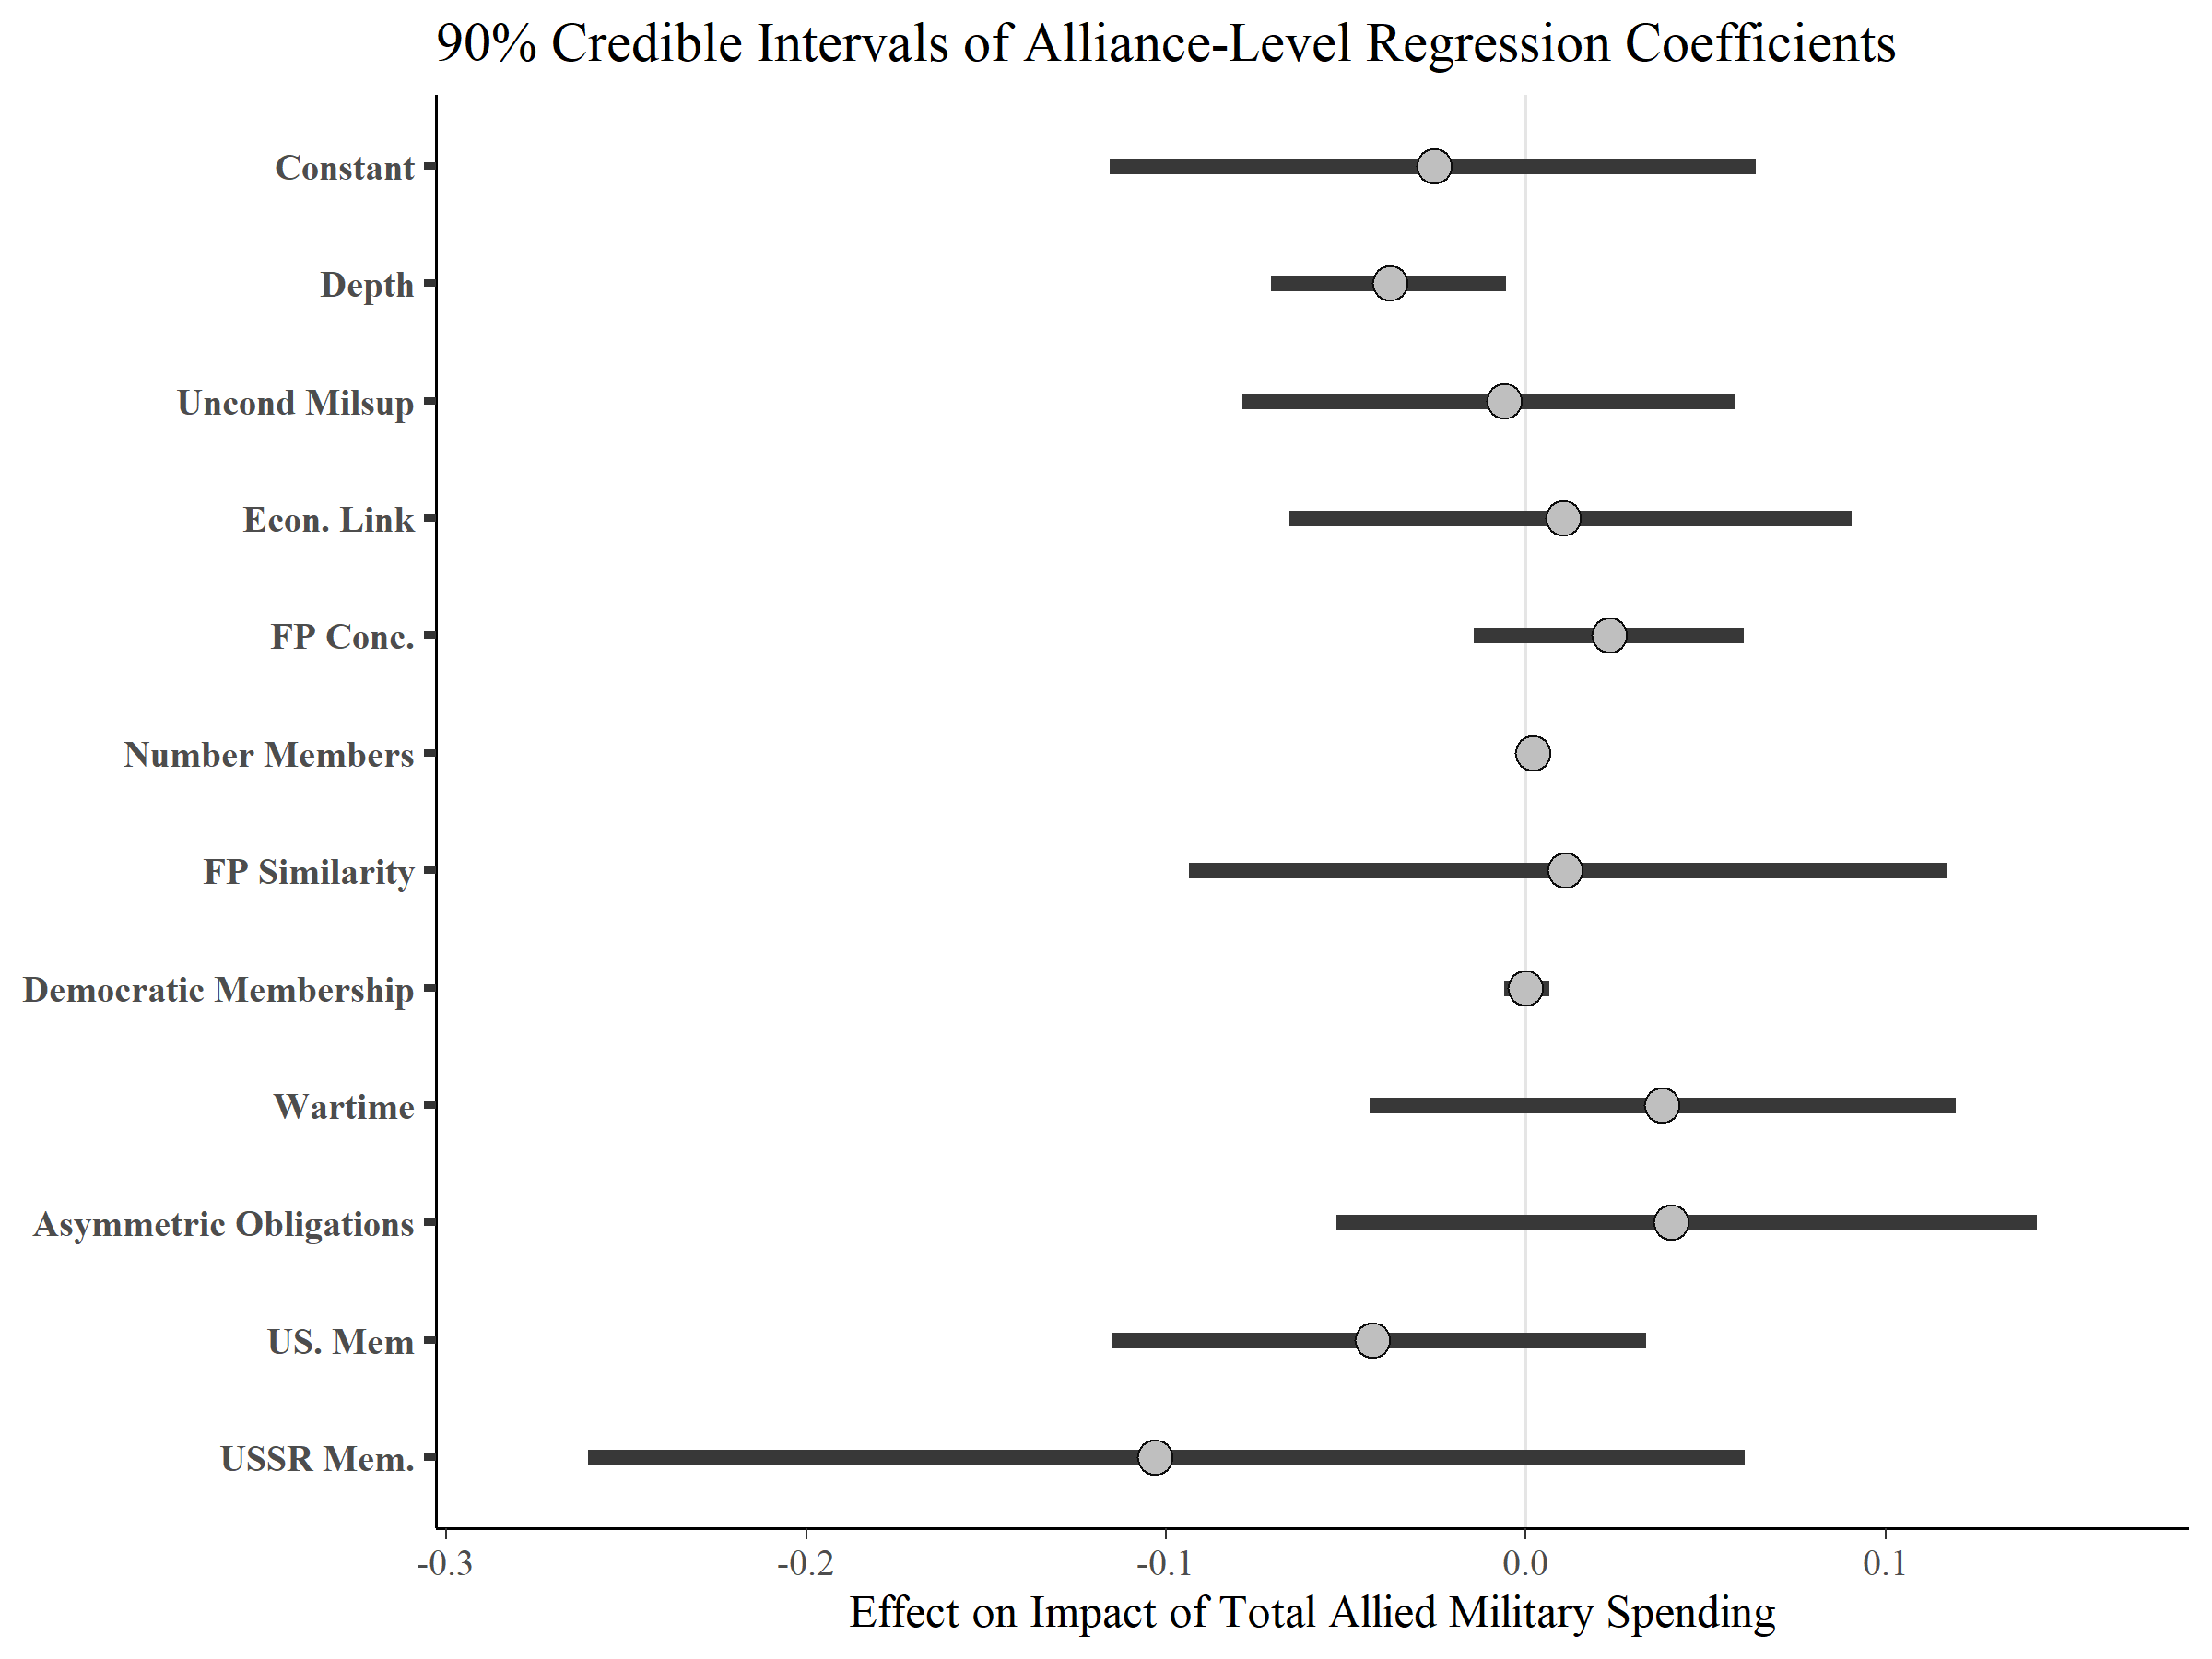
\includegraphics[width=0.95\textwidth]{../figures/alliance-reg-nonmaj.png}
	\caption{90\% credible intervals to summarize the posterior densities of coefficients in the alliance-level regression. Points mark the posterior mean, and the bars encapsulate the width of the credible interval.}
	\label{fig:alliance-reg-nonmaj}
\end{figure}


\
The preponderance of evidence matches the predictions of Hypotheses 1. 
Although the 90\% credible barely overlaps zero, there is a 92\% chance treaty depth is positively associated with growth in military spending for non-major powers.
Treaty depth also has a substantively important effect. 
For non-major powers, the mean of the treaty depth coefficient is 0.02, and median growth in military expenditures is 0.06. 
In expectation, greater treaty depth adds about a third to typical growth in minor power military expenditures.\footnote{Of course, uncertainty in the posterior estimates includes larger and smaller effects.}
This change in spending is a plausible effect--- 5.1\% of the 2018 US defense budget was spent directly on NATO.\footnote{See the following IISS blog post: https://www.iiss.org/blogs/military-balance/2018/07/us-and-nato-allies-costs-and-value.} 


Treaty depth is one of three important correlates of greater defense spending by non-major powers. 
Only wartime alliance obligations and USSR membership in the alliance have a larger posterior mean.
Democratic alliance membership, asymmetric obligations and economic issue linkages all reduce non-major power defense spending.  
The number of members has an unclear effect and there is substantial uncertainty in the superpower dummy estimates. 


%I also assess substantive importance by looking at patterns in the $\lambda$ parameters. 
%Each $\lambda$ measures the impact of treaty participation. 
%If treaty depth has a large influence on alliance participation, it will appear in the $\lambda$ estimates. 
%There should be a positive trend in the expected value of $\lambda$ as treaty depth increases in non-major power alliances.
%On average, shallow alliances should have a more negative effect on members' growth in military spending than deep alliances.  
%
%
%\begin{figure}[htbp]
%	\centering
%		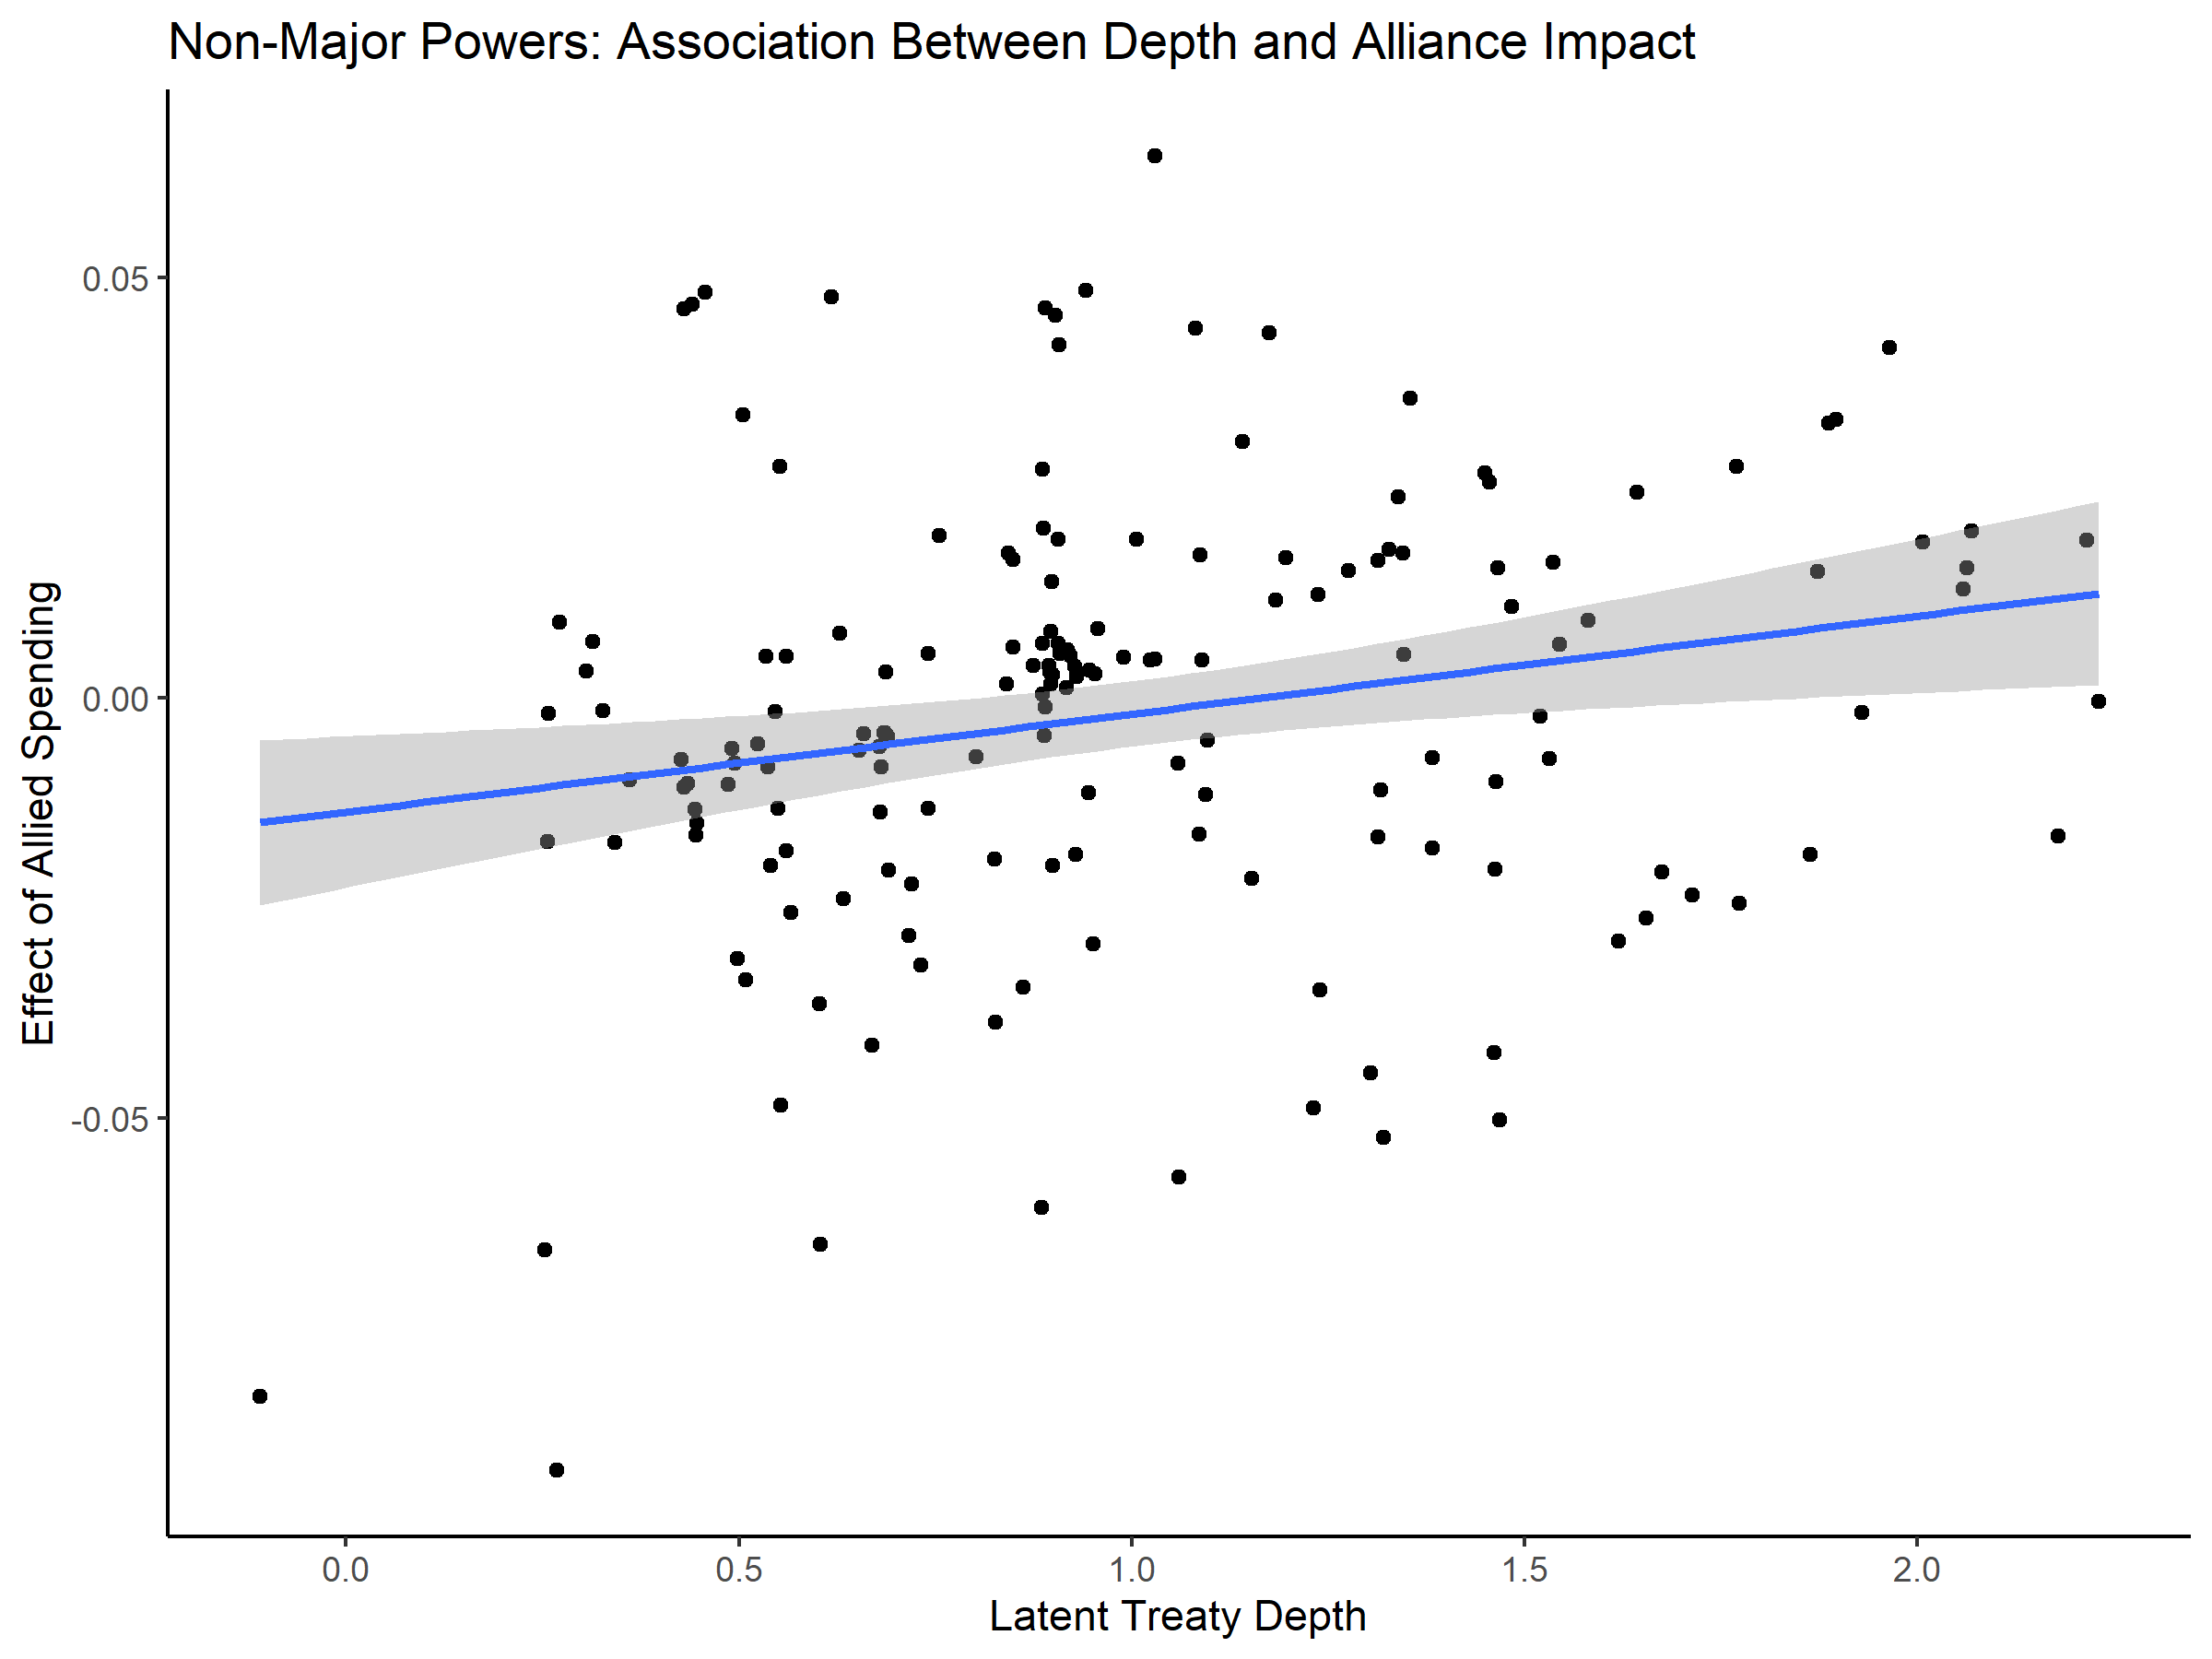
\includegraphics[width=0.95\textwidth]{../figures/lambda-ld-nonmaj-peace.png}
%	\caption{Scatter plots of trends in mean $\lambda$ parameters and treaty depth in peacetime alliances. $\lambda$ is the total impact of alliance participation on growth in military spending. For non-major powers, there is a slight but perceptible increase in $\lambda$ as treaty depth rises. Trend line estimated using linear regression.}
%	\label{fig:lambda-ld-nonmaj-peace}
%\end{figure}
%
%
%\autoref{fig:lambda-ld-nonmaj-peace} plots the expected value of $\lambda$ across the range of treaty depth. 
%For non-major powers, the trend is positive.
%The correlation of .21 between mean $\lambda$ and treaty depth is statistically significant, but of small substantive magnitude. 
%Still, the trend matches the underlying logic of Hypotheses 1. 
%Narrow treaties often reduce growth in military spending among non-major powers, while most broad treaties have a less negative effect. 
%Because other treaty characteristics and unmeasured factors also influence the $\lambda$ estimates, \autoref{fig:lambda-ld-nonmaj-peace} shows tremendous variation in how alliance participation impacts non-major power military spending. 
%Treaty depth is only one source of heterogeneity in how alliance participation impacts military spending. 


The statistical model also allows us to learn about individual alliances. 
Each $\lambda$ parameter captures the impact of an individual alliance. 
Next, I summarize the impact of some US alliances on non-major power defense spending. 


\subsection{US Alliances}


\autoref{fig:depth-impact-us} summarizes the impact of 18 post World War II alliances with US participation on growth in non-major power military spending.
The figure includes both the posterior mean of the $\lambda$ parameter for each alliance and the 90\% credible interval. 
Thirteen of the 18 alliances have a negative mean $\lambda$ estimate. 
Among US alliances, shallow obligations are usually associated with more evidence for a negative impact of the alliance. 


\begin{figure}[htbp]
	\centering
		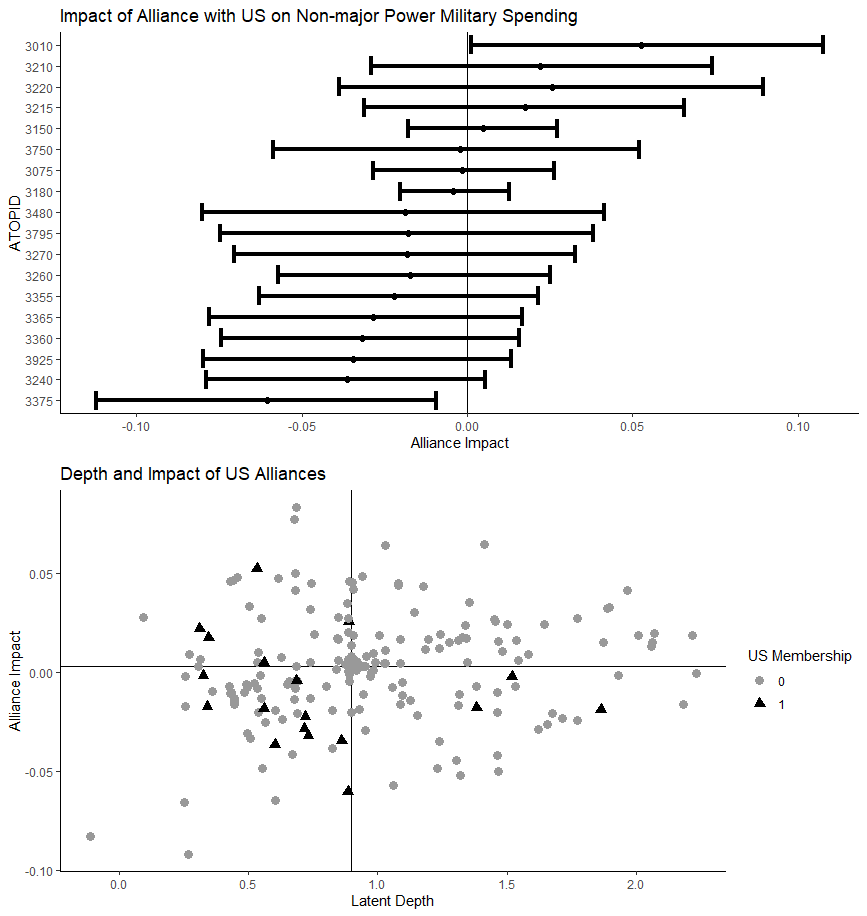
\includegraphics[width=0.95\textwidth]{../figures/depth-impact-us.png}
	\caption{Impact of an alliance with the US on non-major power military spending, 1945-2007. In the top figure, the point summarizes the mean $\lambda$ parameters and the error bars capture the 90\% credible interval. The bottom figure plots the mean $\lambda$ value against the depth of the treaty and highlights US alliances. The vertical and horizontal lines mark the median depth of non-major power alliances and median $\lambda$, respectively.}
	\label{fig:depth-impact-us}
\end{figure}

Most US alliances have limited depth, compared to other treaties. 
Only three US alliances have above average depth, as \autoref{fig:depth-impact-us} shows. 
Ten of eighteen US alliances with non-major powers after 1945 have a below average $\lambda$ as well. 


To further examine the impact of US alliances, I calculated the relative positive or negative posterior probability of each $\lambda$. 
As with regression coefficients, 90\% positive or negative posterior probability is a common threshold for a clear effect. 
One US alliances has a positive $\lambda$ parameter with greater than 90\% positive posterior mass. 
An alliance between the US and other belligerents in World War II (ATOPID 3010). 
The positive effect of this alliance is driven by war.  


There are three US alliances with more than 90\% negative posterior mass in $\lambda$. 
The alliance with Japan (ATOPID 3375) is close to the median alliance in its depth as it scores .89 on the latent measure. 
A formal alliance between the US and Israel from 1981 to 1991 is also close to median depth. 
Last, the US alliance with South Korea (ATOPID 3240) has lower depth. 


Several other alliances have between 75 and 80\% negative posterior mass and below average depth. 
US alliances with Turkey (ATOPID 3360) and Iran (ATOPID 3365)  score around .74 on depth. 
The US alliance with Taiwan (ATOPID 3270) has .58 latent depth, as it includes only a conditional defense obligation.  


% NATO
NATO, the most well-known US alliance, is below average in formal depth. 
The expected impact allied capability on growth in defense spending among non-major powers in NATO is only -0.004, however.\footnote{One possible explanation for this estimate is that it does not include major powers like the UK, France and post-unification Germany that also rely of US protection.}
The small negative effect of NATO reflects extensive defense cooperation outside the formal treaty obligations. 
Defense contacts, regular exercises and bases among NATO members may have limited the negative impact of the alliance on European defense spending. 
Many of these arrangements are outside the formal scope of NATO. 


% Sum it up- limited formal depth to avoid entanglement 
Limited formal depth is standard for US alliances. 
Only one US alliance offers unconditional military support--- a 1963 defense pact with Spain (ATOPID 3480). 
Moreover, few US alliances promise additional defense cooperation. 
US alliances are exemplars of formally arms-length military cooperation \citep{Lake1996}. 


Most defense cooperation with the US takes place through separate agreements outside the formal alliance. 
While constraining the depth of US treaties limits formal entanglement abroad, it also weakens the connection between defense cooperation and the alliance. 
When peacetime cooperation is separated from alliance obligations, non-major power US allies have more freedom to reduce defense expenditures. 



\section{Discussion}


% Precise interpretation: compares alliances. Not treaty vs absence. 
My findings add to our understanding of alliance participation and military spending and address debates over whether alliance participation increases or decreases military spending. 
Claims alliance participation only increases or decreases military spending are inaccurate. 
Treaty depth increases non-major power expenditure growth from alliance participation.\footnote{See the appendix for a robustness check of the multilevel model results with a single-level regression.}
Due to treaty depth and other factors, alliance participation has a wide range of effects on military spending. 


% Link for debate
My argument builds on other conditional arguments about alliance participation and military spending \citep{DigiuseppePoast2016}. 
Non-major powers often reduce military spending, but they cannot reduce growth in military spending in all alliances, because deep treaties constrain.
In some cases, alliance participation clearly increases non-major power military spending, and depth contributes to those positive correlations. 


How do the findings compare to prior evidence on alliance participation and military spending? 
Connecting my results with earlier evidence requires renewed attention to specific and general research designs. 
General studies compare states in an alliance to those without one. 
Specific studies estimate responsiveness to allied military spending in a few treaties. 


The results encompass specific and general studies, as I estimate both the impact of individual treaties and general differences between treaties. 
My research design emulates specific studies by estimating the unique impact of participation in individual treaties. 
The alliance-level coefficients compare treaties to capture the general consequences of alliance characteristics. 


% limitations of RD
This paper has several limitations.
First, the argument offers a cursory treatment of the domestic political economy of military spending, which is itself is the subject of a rich literature \citep{WhittenWilliams2011, AlptekinLevine2012}.  
Furthermore, domestic politics shapes how states define their foreign policy interests and the tools they use to pursue those interests \citep{Fordham1998, Fordham2011, Narizny2007}. 
At the moment, my argument treats foreign policy interests as given.  


My findings also only address formal treaty depth. 
The measure of treaty depth only includes formal promises, in part because informal depth is harder to observe. 
As a result, my test of treaty depth may be conservative--- it does not capture phenomena my argument expects should have a similar effect. 


% Strategic treaty design
Strategic alliance design is another possible weakness of the test. 
Non-random selection into different alliances could produce systematic differences between members that are not captured for in my statistical model. 
I attempted to control for correlates of alliance treaty depth, but oversights are possible.


Despite these limitations, the argument and results provide valuable insights about alliance participation and military spending. 
I explain when alliance participation is associated with more or less growth in military spending among non-major powers, addressing debate between contradictory views of alliances.  
I provide evidence that how alliance participation impacts military spending depends on state capability and alliance treaty depth using a new measure of alliance treaty depth and a multilevel model. 
The argument and findings have implications for scholars and policymakers. 


\section{Conclusion}

% tie it all together
Alliance participation does not uniformly increase or decrease military spending. 
Though alliance participation often reduces non-major power defense spending, spending growth is increasing in alliance treaty depth. 
Alliance participation has a wide range of effects on defense expenditures by non-major powers. 


% Start conclusion
There are several implications of my findings.  
First, they reinforce the importance of accounting for heterogeneity among alliances.
Alliances have heterogeneous effects on the risk of war, trade and military spending \citep{Leeds2003, LongLeeds2006, Benson2012, DigiuseppePoast2016}. 


% Add paragraph on distributional consequences.
Another implication is the distributional consequences of changes in military spending within states and among alliance members.  
By altering growth in military spending, the design of international alliances changes the domestic political economy of member states. 
The economic consequences of alliance participation are a possible subject for future research. 


% The argument indicates tradeoff
Besides their scholarly value, the argument and evidence help inform policy debates. 
Tradeoffs in alliance treaty design can guide our understanding of why some treaties lead to ``free-riding'' and possible policy responses. 
States may be able to check allied free-riding through increasing the depth of their alliance commitments. 
Greater influence requires deeper engagement abroad, however. 


% Implications for policy. 
The United States is currently wrestling with the implications of treaty depth. 
Washington has often decried ``free-riding'' by allies who provide too little for their own defense \citep{Lanoszka2015}. 
But allies are able to free-ride partly because the United States makes shallow formal commitments. 
``Foreign entanglements'' may provide more influence to curb falling allied defense spending. 

 
Therefore, growing institutionalization of NATO, including the agreement for all allies to spend at least 2\% of GDP on defense, should help.
Though defense cooperation within NATO ties the United States more closely to Europe, it is a check on allied free-riding. 
Threatening to leave the alliance undermines whatever benefits the United States receives from its alliances. 

 
This is not an unconditional call for greater depth in US alliance commitments, however. 
Adjusting existing treaties may be more difficult than designing new alliances. 
The full consequences of treaty depth and attempting to change it require additional scrutiny. 

 



\singlespace
 
\bibliography{../../MasterBibliography} 





\end{document}
